\section*{(15\textordfeminine\ aula) --- O Limite Clássico (cap. 6) e o Teorema de Ehrenfest}

\subsection*{O Limite Clássico}

O estado quântico abaixo,
\begin{equation}
    \Psi(x,0) = \frac{e^{ip_0 x/\hbar} \, e^{-(x-x_0)^2/2\Delta^2}}{(\pi \Delta^2)^{1/4}}
\label{eq:aula15_pacote_inicial}
\end{equation}
tem $\langle X \rangle = x_0$, $\Delta X = \dfrac{\Delta}{\sqrt{2}}$, $\langle P \rangle = p_0$ e $\Delta P = \dfrac{\hbar}{\sqrt{2}\Delta}$. Esse estado pode ser pensado como a melhor versão quântica da partícula clássica.

Vimos que se $\Delta X \sim 10^{-15}\,\text{m}$ temos $\Delta P \sim 10^{-19}\,\text{kg}\cdot\text{m/s}$, que para uma partícula de massa $m = 1\,\text{g}$ implica em uma velocidade conhecida com precisão de $\Delta V = \dfrac{\Delta P}{m} \sim 10^{-16}\,\text{m/s}$, maior precisão que qualquer instrumento de medida pode proporcionar.

Vimos também que esse estado, na ausência de forças, evolui para
\begin{equation}
    |\Psi(x,t)|^2 = \frac{1}{\sqrt{\pi}\,\Delta(t)} \exp\left[ -\frac{(x - x_0 - p_0 t/m)^2}{\Delta(t)^2} \right]
\label{eq:aula15_pacote_evoluido}
\end{equation}
com
\begin{equation}
    \Delta(t) = \sqrt{\Delta^2 + \frac{\hbar^2 t^2}{m^2 \Delta^2}},
\label{eq:aula15_delta_t}
\end{equation}
a largura do pacote, crescendo muito lentamente para $m \sim 1\,\text{g}$.

Concluímos que, para uma partícula livre, a Eq. de Schrödinger contém o resultado clássico da partícula se movendo com velocidade constante $p_0/m$ e $|\Psi(x,t)|^2$ tem características de "partícula" (não apresentando alargamento do pacote).

\subsection*{Teorema de Ehrenfest}

Vamos agora derivar o \textbf{Teorema de Ehrenfest} e ver como exatamente $F = ma$ se esconde na Eq. de Schrödinger.

Seja um operador $\hat{\Omega}$, independente do tempo, e um estado $\ket{\Psi(t)}$ que evolui de acordo com a E.S.
\begin{equation}
    i\hbar \frac{d}{dt}\ket{\Psi(t)} = \hat{H}\ket{\Psi(t)}.
\label{eq:aula15_eq_schrodinger}
\end{equation}

O valor médio de $\hat{\Omega}$ muda com o tempo de acordo com
\begin{equation}
    \frac{d}{dt}\bra{\Psi(t)}\hat{\Omega}\ket{\Psi(t)} = \left[\frac{d}{dt}\bra{\Psi}\right]\hat{\Omega}\ket{\Psi} + \bra{\Psi}\hat{\Omega}\left[\frac{d}{dt}\ket{\Psi}\right].
\label{eq:aula15_dOmega_1}
\end{equation}

Tome o adjunto da E.S. para encontrar
\begin{equation}
    -i\hbar \frac{d}{dt}\bra{\Psi} = \bra{\Psi}\hat{H}.
\label{eq:aula15_adjunto_es}
\end{equation}

Substituindo as derivadas de $\bra{\Psi}$ e $\ket{\Psi}$ usando a E.S. e seu adjunto,
\begin{equation}
    \frac{d}{dt}\aver{\hat{\Omega}} = \frac{i}{\hbar}\bra{\Psi}\hat{H}\hat{\Omega}\ket{\Psi} - \frac{i}{\hbar}\bra{\Psi}\hat{\Omega}\hat{H}\ket{\Psi}.
\label{eq:aula15_dOmega_2}
\end{equation}

\begin{equation}
    \boxed{\frac{d\aver{\hat{\Omega}}}{dt} = \frac{1}{i\hbar}\bra{\Psi}[\hat{\Omega}, \hat{H}]\ket{\Psi}} \qquad \text{(Teorema de Ehrenfest)}
\label{eq:aula15_ehrenfest}
\end{equation}

Compare isso com a relação da Mecânica Hamiltoniana
\begin{equation}
    \frac{d}{dt}w(p,q) = \{w, H\} = \frac{\partial w}{\partial q}\frac{\partial H}{\partial p} - \frac{\partial w}{\partial p}\frac{\partial H}{\partial q}.
\label{eq:aula15_poisson_comparacao}
\end{equation}

Usando $\hat{\Omega} = \hat{X}$ temos
\begin{equation}
    \frac{d\aver{\hat{X}}}{dt} = \frac{1}{i\hbar}\aver{[\hat{X}, \hat{H}]}.
\label{eq:aula15_dX_ehrenfest}
\end{equation}

\subsection*{Aplicação: $\hat{H} = \dfrac{\hat{P}^2}{2m} + V(\hat{X})$}

Se $\hat{H} = \dfrac{\hat{P}^2}{2m} + V(\hat{X})$, então
\begin{equation}
    [\hat{X}, \hat{H}] = \left[\hat{X}, \frac{\hat{P}^2}{2m}\right] + [\hat{X}, V(\hat{X})] = \frac{i\hbar}{m}\hat{P}.
\label{eq:aula15_comutador_X_H}
\end{equation}

Aqui usei a propriedade de comutadores (1.5.10):
\begin{equation}
    [\hat{X}, \hat{P}^2] = \hat{P}\underbrace{[\hat{X}, \hat{P}]}_{i\hbar} + \underbrace{[\hat{X}, \hat{P}]}_{i\hbar}\hat{P} = 2i\hbar\hat{P}.
\label{eq:aula15_comutador_X_P2}
\end{equation}

Portanto
\begin{equation}
    \boxed{\frac{d\aver{\hat{X}}}{dt} = \frac{\aver{\hat{P}}}{m}}
\label{eq:aula15_dX_dt_resultado}
\end{equation}
ou seja, a taxa de variação do valor médio de $\hat{X}$ é igual ao valor médio de $\hat{P}/m$.

Usando agora $\hat{\Omega} = \hat{P}$ no Teorema de Ehrenfest encontro
\begin{equation}
    \frac{d\aver{\hat{P}}}{dt} = \frac{1}{i\hbar}\aver{[\hat{P}, \hat{H}]},
\label{eq:aula15_dP_ehrenfest}
\end{equation}
e usando $\hat{H} = \dfrac{\hat{P}^2}{2m} + V(\hat{X})$ temos $\dfrac{1}{i\hbar}[\hat{P}, \hat{H}] = \dfrac{1}{i\hbar}[\hat{P}, V(\hat{X})]$.

\subsection*{Comutadores $[\hat{P}, V(\hat{X})]$ e $[\hat{X}, f(\hat{P})]$}

Sempre que encontrar $[\hat{P}, V(\hat{X})]$ ou $[\hat{X}, f(\hat{P})]$ use o resultado
\begin{equation}
    [\hat{P}, \hat{X}^n] = (-i\hbar)\, n\, \hat{X}^{n-1}, \qquad [\hat{X}, \hat{P}^n] = (i\hbar)\, n\, \hat{P}^{n-1},
\label{eq:aula15_comutadores_potencias}
\end{equation}
que é demonstrado por \textbf{indução}:
\begin{enumerate}
    \item[(i)] As expressões são válidas para $n = 1$ (cheque).
    \item[(ii)] Se as expressões são válidas para $n$, elas também valerão para $n+1$.
\end{enumerate}

Veja como o passo (ii) se verifica:
\begin{equation}
    [\hat{P}, \hat{X}^n] = (-i\hbar)\, n\, \hat{X}^{n-1} \quad \text{(válido por hipótese)}
\label{eq:aula15_inducao_hipotese}
\end{equation}

\begin{align}
    [\hat{P}, \hat{X}^{n+1}] &= \hat{X}\,[\hat{P}, \hat{X}^n] + [\hat{P}, \hat{X}]\,\hat{X}^n \qquad \text{(prop. dos comutadores)} \notag \\
    &= \hat{X}(-i\hbar)\, n\, \hat{X}^{n-1} + (-i\hbar)\hat{X}^n \qquad \text{(usando a hipótese e } [\hat{P}, \hat{X}] = -i\hbar\text{)} \notag \\
    &= (-i\hbar)(n+1)\,\hat{X}^n \qquad \text{(verificando a validade da fórmula para } n+1\text{)}.
\label{eq:aula15_inducao_passo}
\end{align}

Agora use a definição $V(\hat{X}) = \displaystyle\sum_{n=0}^{\infty} a_n \hat{X}^n$ para concluir
\begin{align}
    [\hat{P}, V(\hat{X})] &= \sum_{n=0}^{\infty} a_n [\hat{P}, \hat{X}^n] = \sum_{n=1}^{\infty} a_n (-i\hbar)\, n\, \hat{X}^{n-1} \notag \\
    &= (-i\hbar)\frac{dV}{d\hat{X}}
\label{eq:aula15_comutador_P_V}
\end{align}
onde $\dfrac{dV}{d\hat{X}}$ representa o operador obtido derivando $V(\hat{X})$ como se fosse uma função normal da variável $\hat{X}$. Assim:
\begin{equation}
    \boxed{[\hat{P}, V(\hat{X})] = -i\hbar \frac{dV}{d\hat{X}}} \qquad \boxed{[\hat{X}, f(\hat{P})] = i\hbar \frac{df}{d\hat{P}}}
\label{eq:aula15_comutadores_gerais}
\end{equation}
(a segunda relação se demonstra da mesma forma).

\textbf{Ex.:} $[\hat{P}, \sin \hat{X}] = (-i\hbar)\cos\hat{X}$ e $[\hat{X}, e^{\hat{P}}] = i\hbar\, e^{\hat{P}}$.

Dessa forma:
\begin{equation}
    \frac{d\aver{\hat{P}}}{dt} = \aver{-\frac{dV}{d\hat{X}}} = \aver{F(\hat{X})}
\label{eq:aula15_dP_dt_resultado}
\end{equation}
onde $-\dfrac{dV}{d\hat{X}}$ é o \textbf{operador força}.

A taxa de variação do valor médio de $\hat{P}$ é igual ao valor médio do operador força.

\subsection*{$\aver{X(t)}$ obedece a Equação de Newton?}

Obtemos as equações clássicas apenas para os valores médios.

Essas duas equações para $\aver{X}$ e $\aver{P}$ implicam que o valor médio $\aver{X(t)}$ obedece à Eq. de Newton?

\textbf{Não!} Pois para isso acontecer deveríamos ter obtido:
\begin{equation}
    \frac{d\aver{\hat{X}}}{dt} = \frac{\aver{\hat{P}}}{m} \quad \text{e} \quad \frac{d\aver{\hat{P}}}{dt} = F(\aver{\hat{X}}) \quad \Longrightarrow \quad m\frac{d^2\aver{\hat{X}}}{dt^2} = F(\aver{\hat{X}}),
\label{eq:aula15_newton_desejado}
\end{equation}

no entanto obtivemos:
\begin{equation}
    \frac{d\aver{\hat{X}}}{dt} = \frac{\aver{\hat{P}}}{m} \quad \text{e} \quad \frac{d\aver{\hat{P}}}{dt} = \aver{F(\hat{X})} \quad \Longrightarrow \quad m\frac{d^2\aver{\hat{X}}}{dt^2} = \aver{F(\hat{X})}.
\label{eq:aula15_newton_obtido}
\end{equation}

Qual a diferença entre $F(\aver{\hat{X}})$ e $\aver{F(\hat{X})}$? Uma é a força clássica avaliada em $\aver{\hat{X}}$, a outra é a média da força clássica sobre toda a função de onda da partícula.

\begin{equation}
    \aver{F(\hat{X})} = \int_{-\infty}^{\infty} |\Psi(x,t)|^2 F(x) \, dx \quad \neq \quad F\left(\int_{-\infty}^{\infty} |\Psi(x,t)|^2 x \, dx\right) = F(x_0), \qquad \aver{\hat{X}} \equiv x_0.
\label{eq:aula15_F_media_vs_F_de_media}
\end{equation}

Usando a série de Taylor de $F(x)$ em torno do valor médio $\aver{\hat{X}} \equiv x_0$ temos
\begin{align}
    \aver{F(\hat{X})} &= \int_{-\infty}^{\infty} |\Psi(x,t)|^2 \left[ F(x_0) + F'(x_0)(x - x_0) + \frac{1}{2}F''(x_0)(x-x_0)^2 + \dots \right] dx \notag \\
    &= F(x_0) + F'(x_0)\underbrace{(x_0 - x_0)}_{0} + \frac{1}{2}F''(x_0)\underbrace{\left(\aver{\hat{X}^2} - x_0^2\right)}_{\Delta X^2} + \dots
\label{eq:aula15_taylor_F}
\end{align}

\begin{center}
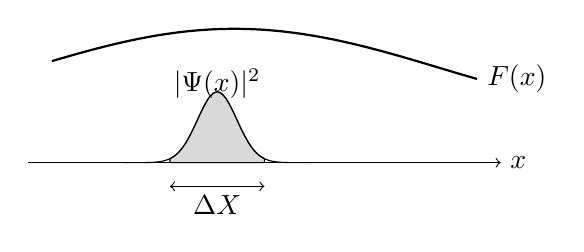
\begin{tikzpicture}[scale=1]
    \draw[->] (0,0) -- (6,0) node[right] {$x$};
    \draw[domain=0.3:5.7, smooth, variable=\x, thick] plot ({\x}, {1.2+0.5*sin(0.6*\x r)}) node[right] {$F(x)$};
    \draw[domain=1.8:3.0, smooth, variable=\x, fill=gray!30] plot ({\x}, {0.9*exp(-8*(\x-2.4)*(\x-2.4))}) -- (3.0,0) -- (1.8,0) -- cycle;
    \draw[domain=1.2:3.6, smooth, variable=\x] plot ({\x}, {0.9*exp(-8*(\x-2.4)*(\x-2.4))});
    \draw[<->] (1.8,-0.3) -- (3.0,-0.3) node[midway, below] {$\Delta X$};
    \node at (2.4,1.0) {$|\Psi(x)|^2$};
\end{tikzpicture}
\end{center}

Nesse desenho $F(x)$ não varia apreciavelmente na escala $\Delta X$.

Portanto, se a força não varia apreciavelmente em uma distância da ordem da largura de $\Psi$, $\Delta X$:
\begin{equation}
    \underbrace{F(x_0) \gg F''(x_0)\,\Delta X^2 \quad \Longrightarrow \quad \aver{F(\hat{X})} \sim F(\aver{\hat{X}})}_{(*)},
\label{eq:aula15_condicao_estrela}
\end{equation}
e $\aver{X(t)}$ obedece $F = ma$!

\subsection*{Discussão: massas pequenas vs. massas grandes}

Se na função de onda gaussiana do início da aula temos $\Delta X \sim 10^{-15}\,\text{m}$, e a partícula associada tem massa $m \sim 1\,\text{g}$, $\Delta V \sim 10^{-16}\,\text{m/s}$. Como é essencialmente a incerteza na velocidade da partícula que leva ao alargamento do pacote, $\Delta X$ permanece pequeno e a condição acima é certamente válida por longos tempos $\Rightarrow$ o valor médio $\aver{X}$ segue a trajetória ditada por $F = ma$. Como o pacote permanece estreito, a função de onda \textbf{É} a partícula clássica, com posição e velocidade bem definidas.

Com esse mesmo estado, caso $m \sim m_e$ (massa do elétron), a incerteza na velocidade seria $\Delta V \sim 10^{12}\,\text{m/s}$ e o pacote se alargaria muito rapidamente, rapidamente invalidando a condição $(*)$ acima. O valor médio $\aver{\hat{X}}$ não seguiria a trajetória clássica.

\textbf{Caso $m \sim 1\,\text{g}$:} não há alargamento, e $\aver{X}$ obedece $F = ma$ — a partícula segue uma trajetória clássica bem definida.

\textbf{Caso $m \sim m_e$:} há alargamento do pacote (ilustrado por duas regiões sobrepostas, alargadas e irregulares, centradas na trajetória), e $\aver{X}$ não obedece $F = ma$.

\subsection*{Caso do potencial harmônico}

No caso do potencial harmônico $V(x) = \dfrac{1}{2}m\omega^2 x^2$, a força é a lei de Hooke $F(x) = -m\omega^2 x$ e $F''(x) = 0$, portanto a condição $(*)$ é sempre satisfeita, \textbf{independente do tamanho de $\Delta X$}.

Aqui, mesmo para partículas leves, $\aver{X}$ segue $F = ma$, isto é
\begin{equation}
    m\frac{d^2\aver{X}}{dt^2} = -m\omega^2 \aver{X}.
\label{eq:aula15_newton_harmonico}
\end{equation}

A diferença entre uma partícula leve e uma pesada está em que a primeira exibe o alargamento do pacote enquanto a segunda não.

\subsection*{Potenciais descontínuos}

No caso dos potenciais descontínuos que já discutimos, a variação abrupta do potencial faz com que a condição $(*)$ não seja satisfeita mesmo para $\Delta X$ muito pequeno. $\Rightarrow$ $\aver{X}$ não obedece $F = ma$ nesses casos.

\textbf{Ex.:} No caso do poço infinito vimos a simulação da dinâmica de um pacote gaussiano. Observamos desvios de $\aver{X(t)}$ da trajetória clássica nas proximidades das paredes.

\begin{center}
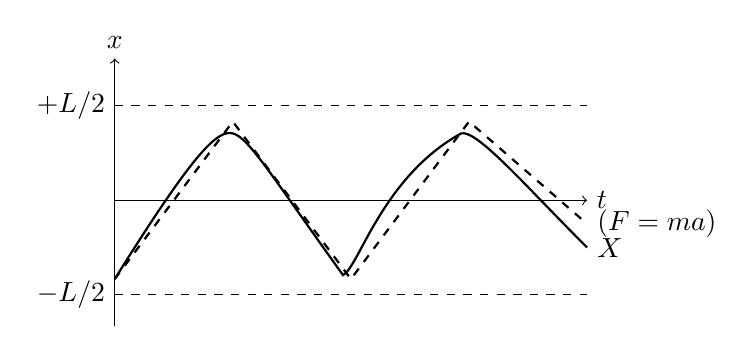
\begin{tikzpicture}[scale=1]
    \draw[->] (0,0) -- (6,0) node[right] {$t$};
    \draw[->] (0,-1.6) -- (0,1.8) node[above] {$x$};
    \node[left] at (0,1.2) {$+L/2$};
    \node[left] at (0,-1.2) {$-L/2$};
    \draw[dashed] (0,1.2) -- (6,1.2);
    \draw[dashed] (0,-1.2) -- (6,-1.2);
    \draw[dashed, thick] (0,-1.0) -- (1.5,1.0) -- (3.0,-1.0) -- (4.5,1.0) -- (6,-0.3) node[right] {$(F=ma)$};
    \draw[thick] (0,-1.0) .. controls (1.0,0.6) and (1.3,0.9) .. (1.5,0.85) .. controls (1.7,0.8) and (2.0,0.3) .. (2.9,-0.95) .. controls (3.1,-0.85) and (3.4,0.3) .. (4.4,0.85) .. controls (4.6,0.9) and (5.2,0.2) .. (6,-0.6) node[right] {$\aver{X}$};
\end{tikzpicture}
\end{center}

\textbf{Ex.:} No caso de um pacote incidindo em um degrau com $\aver{E} > V_0$ (classicamente a partícula não seria refletida):

\begin{center}
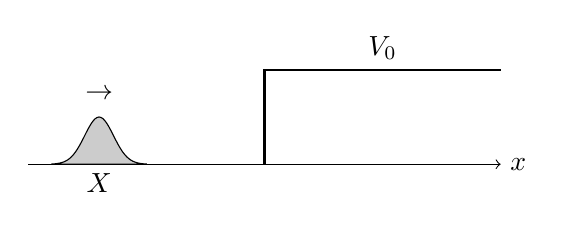
\begin{tikzpicture}[scale=1]
    \draw[->] (0,0) -- (6,0) node[right] {$x$};
    \draw[thick] (3,0) -- (3,1.2) -- (6,1.2);
    \node[above] at (4.5,1.2) {$V_0$};
    \draw[domain=0.3:1.5, smooth, variable=\x, fill=gray!40] plot ({\x}, {0.6*exp(-15*(\x-0.9)*(\x-0.9))}) -- (1.5,0) -- (0.3,0) -- cycle;
    \node[below] at (0.9,0) {$\aver{X}$};
    \node[above] at (0.9,0.7) {$\rightarrow$};
\end{tikzpicture}
\hspace{1cm}
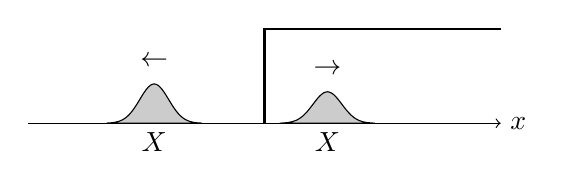
\begin{tikzpicture}[scale=1]
    \draw[->] (0,0) -- (6,0) node[right] {$x$};
    \draw[thick] (3,0) -- (3,1.2) -- (6,1.2);
    \draw[domain=1.0:2.2, smooth, variable=\x, fill=gray!40] plot ({\x}, {0.5*exp(-15*(\x-1.6)*(\x-1.6))}) -- (2.2,0) -- (1.0,0) -- cycle;
    \node[above] at (1.6,0.6) {$\leftarrow$};
    \draw[domain=3.2:4.4, smooth, variable=\x, fill=gray!40] plot ({\x}, {0.4*exp(-15*(\x-3.8)*(\x-3.8))}) -- (4.4,0) -- (3.2,0) -- cycle;
    \node[above] at (3.8,0.5) {$\rightarrow$};
    \node[below] at (1.6,0) {$\aver{X}$};
    \node[below] at (3.8,0) {$\aver{X}$};
\end{tikzpicture}
\end{center}

Após a colisão com o degrau, $\aver{X}$ avança mais lentamente (devido ao pacote refletido) que o previsto por $F = ma$.

\subsection*{Conclusão}

\fbox{\parbox{0.92\textwidth}{
Em suma: para se observar $F = ma$ na Eq. de Schrödinger há dois pontos a considerar.

\begin{enumerate}
    \item Um pacote "clássico" como o $\Psi(x)$ do início da aula deve se manter estreito durante a evolução do sistema (isso ocorre com \textbf{massas grandes}).
    \item O potencial deve ser tal que, para o $\Delta X$ do pacote, $F''(\aver{X})\,\Delta X^2 \ll F(\aver{X})$ se verifique. Isso implica que $\aver{X}$ seguirá a trajetória clássica determinada por $F = ma$.
\end{enumerate}

Caso essas duas condições se verifiquem, a descrição quântica do problema em questão é \textbf{desnecessária}. Basta usar $F = ma$.
}}
